\chapter{Large Language Models}\label{ch:techOverview}

Creating machines with human-like language understanding has been a subject of research since the 1950s.
\gls{natural-language}s are highly complex and pose a difficult challenge to computers.
% ambiguous: ~\autocite{quadarLM2020}
\gls{lm} is an approach to make machines read, write and communicate like humans~\autocite{zhao2023survey}.

The main idea of \gls{lm} is to estimate probability distributions over units of texts, e.g.\ words~\autocite{de2015survey}.
Assuming that the occurrence of a word depends on previous words, i.e.\ the context, the probability of that word being next in a sentence can be modeled with a conditional probability~\autocite{jozefowicz2016exploring}.
\[
    P(w_n | w_1, \dots , w_{n-1})
\]
% TODO: quelle finden vielleicht
The ability to estimate the probability distributions over words makes it possible to predict the next word for a given sequence.
In this way, language models can be applied in many \gls{nlp} tasks like speech recognition, machine translation and text summarization~\autocite{jozefowicz2016exploring}.
By simply predicting the next word, language models can hold human-like conversations, which makes it appear as if they understand natural language.
% How would translation look like?
% TODO: Other approaches like BERT Masked language Modeling
%Other approaches to \gls{lm} mask parts of sentences and use all surrounding language units to predict the missing

There are different techniques to model these probabilities of word sequences.
In the 1990s, \glspl{slm} found widespread use.
The models often assume that the distribution of a word only depends on a fixed length of previous words.
\enquote{$n$-grams models} are \glspl{slm} that use the previous $n$ words to calculate the probability distribution of the next word.
Based on a training corpus, tables of conditional probabilities are created.
The probabilities are approximated by counting occurrences of $n$-grams.
If the previous word is \enquote{thank}, the probability that the next word is \enquote{you} could be estimated as follows~\autocite{quadarLM2020}
\[
    P(\text{you} | \text{thank}) = \frac{P(\text{thank you})}{P(\text{thank})} \approx \frac{count(\text{thank you})}{count(\text{thank})}
\]
In recent years, research has been focused on the more flexible \glspl{nlm}~\autocite{quadarLM2020}.
This approach uses \glspl{dnn} to estimate the needed probability distributions.
\glspl{nlm} are much better at taking long-range depencies in text into account than \glspl{slm}~\autocite{Hadi_2023}.
\glspl{dnn} excel at extracting complex features from text and finding meaningful representations for words.
These representations (often called embeddings) lie in a vector space of real vectors where similar words are close to each other in a mathematical sense~\autocite{quadarLM2020}.
In \glspl{nlm} the prediction function is usually built on top of these embeddings.
The intermediate step of learning effective features and representing them in embeddings has the benefit that those embeddings can be reused for other tasks.
The early 2010s saw the rise of \glspl{dnn} that were specifically designed to create powerful word embeddings~\autocite{zhao2023survey}.
These embeddings were static, meaning the network would assign each word exactly one embedding, disregarding polysemy of words~\autocite{Liu_2020}.
Embeddings of popular solutions like \enquote{word2vec} proved to be very useful in various \gls{nlp}-Tasks.

Following research focused on incorporating context into word embeddings, i.e.\ assigning a different vector representation to a word depending on the surrounding words.
ELMo, BERT and GPT are well-known models that managed to do so.
These context-aware language models are trained on large unlabeled corpora of text data.
During training, the models learn to solve pre-training tasks that are specifically designed for the language model to gain essential language understanding.
They are often put into their own class of language models, the so-called \glspl{plm}.
\glspl{plm} set new standards in solutions of many \gls{nlp}-tasks.

They learn general-purpose features that are u

%With the introduction of the transformer architecture in 2017~\autocite{vaswani2023attention}


\section{notes}

\begin{figure}
    \centering
    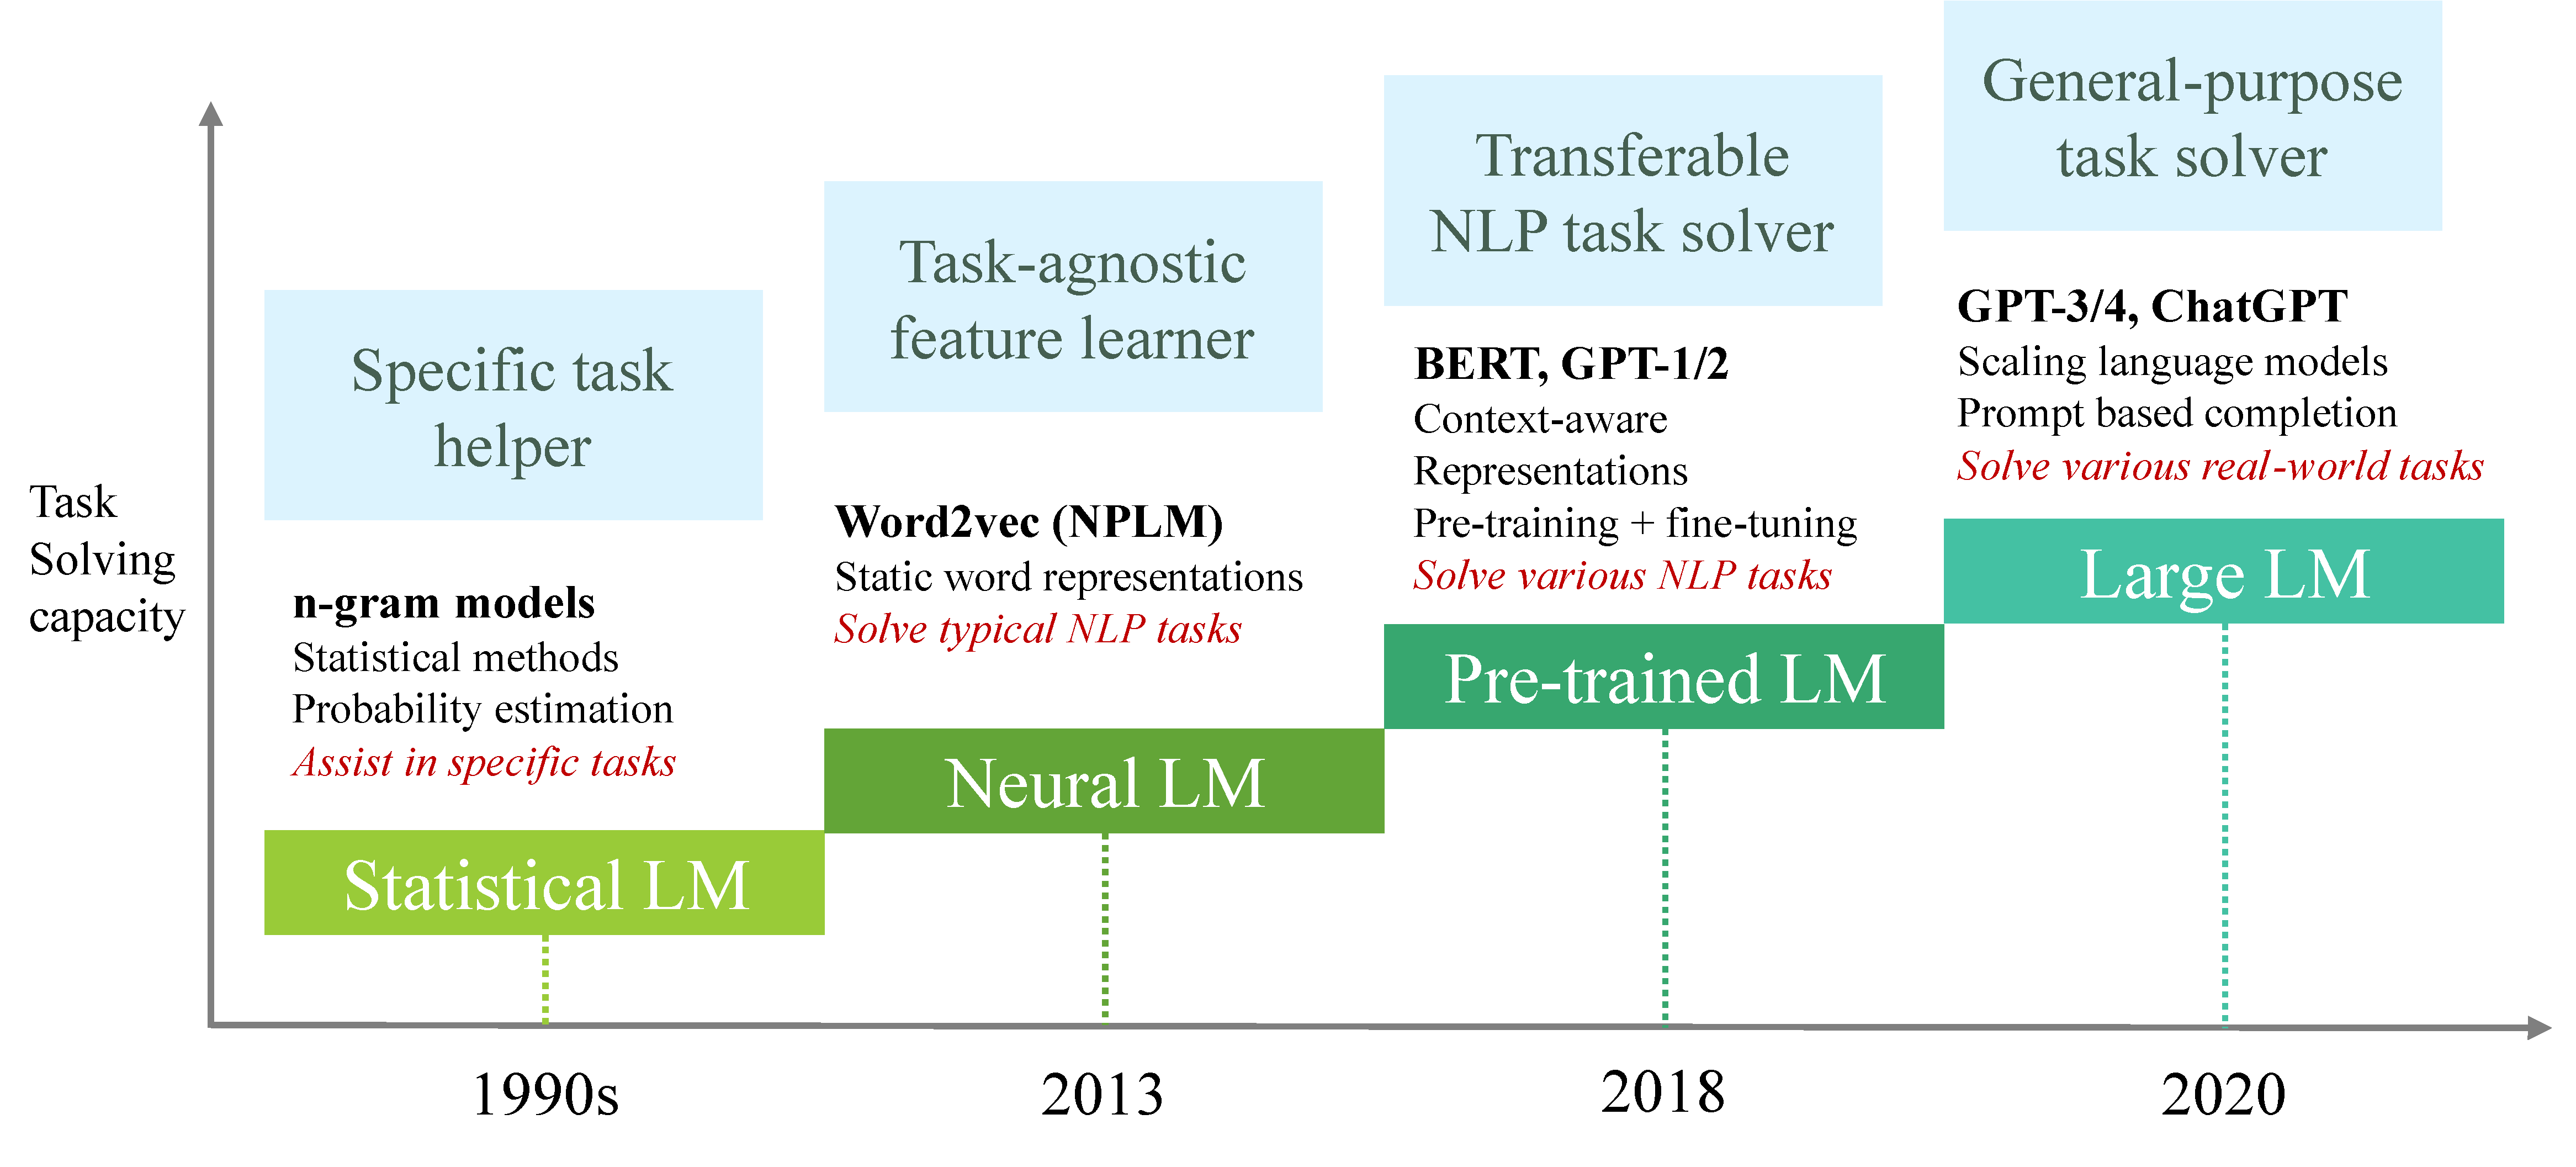
\includegraphics[width=\linewidth]{images/languagemodels}
    \caption[TODO.]{TODO}
    \label{fig:language-models}
\end{figure}

from~\autocite{zhao2023survey}:

Pre-trained language models (PLM) -> context-aware word representations (versatile, usable for various tasks)
learning general purpose features (pre-training and fine-tuning) -> (GPT 2)
fine-tuning is necessary

Large Language Models (LLM) -> scaling PLMs improves performance (bigger more complex models)
surprising abilities (emergent abilities)
solve complex tasks without fine-tuning
ChatGPT with amazing conversation abilities

task-agnostic representations -> less human feature engineering

from ~\autocite{Raiaan2024ARO}:
pre-training on large corpora from the web -> learning complicated patterns and language subtleties
fine-tuning on downstream tasks gives state-of-the-art performance
neural language model in 2010s
"comprehend, produce, forecast human language"
BERT and GPT as miles-stones (attention)
improved performance by scaling up models
pre-training with extensive datasets

From ~\autocite{Hadi_2023}:
\gls{llm}s result of rise of deep learning, availability of huge datasets, powerful computing devices
\gls{llm} usually refers to lm with transformer architecture
understanding context
breakthrough for llm: "attention is all you need"
during pre-training: models see diverse texts and learn grammar, facts, reasoning
fine-tuning for more specific task ("narrow dataset")

from~\autocite{Liu_2020}:
representation learning

from~\autocite{bhatia2023tart}:
in-context learning of LLMs: perform tasks given only a few examples, not updating model parameters
impressive results but usually still outperformed by fine-tuning

\section{Deep Neural Networks}\label{sec:dnn}

\subsection{Multi Layer Perceptron}\label{subsec:multi-layer-perceptron}

\subsection{Learning from Data (Gradient Descent)}\label{subsec:learning-from-data}
% Mathematical Optimization

\subsubsection{Loss Functions}

\subsubsection{Backpropagation}

\section{Transformers}\label{sec:trans}

\section{Decoder-only Models}\label{sec:decoder}

\subsection{GPT}\label{subsec:gpt}

\subsection{Llama}\label{subsec:llama}

\subsubsection{Leo}

\section{Supervised Fine-Tuning (SFT)}\label{sec:supervised-fine-tuning}

\section{Alignment Methods}\label{sec:alignment-methods}
from~\autocite{zhao2023survey}:
capture properties of training corpus

\subsection{RLHF}\label{subsec:rlhf}
\subsection{PPO}\label{subsec:ppo}
\subsection{DPO}\label{subsec:dpo}
